\section{Classified Image Based Performance Evaluation}  \label{section:classifiedeval}

\subsection{Image-based VTON}

In this Section, we start with evaluating the 2D image-based virtual try-on (VTON) algorithms. We consider CP-VTON\cite{Wang2018TowardCI} published in 2018 as the benchmark algorithm. Most of the recently proposed image-based approaches\cite{Han2017VITONAI,Sun2019ImageBasedVT,Yu_2019_ICCV} share same input images and information conditions as CP-VTON and compare the results with it. Here, we include the comparison among Shape-Context Matching (SCM) based-VTON, VITON\cite{Han2017VITONAI}, and  CP-VTON\cite{Wang2018TowardCI}. However, we believe the performance strengths and weaknesses are similar in other recently proposed algorithms as well.


The Image based virtual try-on algorithms are mostly composed of two stages: (1) cloth warping step that warps the try-on cloth to align with the pose and shape of the target model (called GMM in CP-VTON: Geometric Matching Module)\cite{Wang2018TowardCI}, and (2) blending step that blends the warped cloth onto the target human image (called TOM in CP-VTON: Try-On Module)\cite{Wang2018TowardCI}. CP-VTON\cite{Wang2018TowardCI} assumes the target human image is pre-processed for a cloth agnostic human representation by a human pose estimation e.g. OpenPose\cite{Cao2018OpenPoseRM}, and human parsing e.g. LIP\cite{Liang2018LookIP}. The human representation is composed of 1) heat-maps for each joints 2) silhouette of human body, and 3) face and skin pixels patches (non-clothing and human identity area). We use the same dataset collected by Han et al. used in VITON\cite{Han2017VITONAI} and CP-VTON\cite{Wang2018TowardCI} papers.


\subsection{Classified quality}

Even though the success and failure cases are presented and compared with other algorithms' results, the failure cases' analysis are not enough for understanding the origin of failure cases, and its difficult to find the solutions from the presented results. Therefore, we believe that a classified evaluation would be better for getting better understanding of the baseline algorithms. Here, we summarized the classified comparison results on the state-of-the-art image-based virtual try-on approaches. We classified input try-on cloth and target human images according to the postures and body shape types of human models, degree of occlusions of the outfit clothing, and the characteristics of the fashion clothing. For the same cloth re-try-on, we compared the qualities by using the metrics Intersection-over-Union (IoU) for the warping try-on clothing stage, and Structural Similarity Index (SSIM) for the final blending stage. Although in general, CP-VTON\cite{Wang2018TowardCI} generates the best quality results, the relative comparison is not the main purpose of our classified analysis. Please refer to Figure \ref{fig:classified2DVTONresult} for same clothes and Figure \ref{fig:2dvtondiff} for different clothes try-on results.

% We compared the cases where the target human models are wearing the same clothes as in the try-on clothes, so that we could measure the metric values with ground truths. We also tested for different clothes try-on cases. However, we did not include the figures here for the sake of keeping the comparison shorter, and we believe the same clothing input image pair cases are sufficient to explain the tendencies of the performances in the state-of-the-art models. 



\begin{figure}[t]
\centering
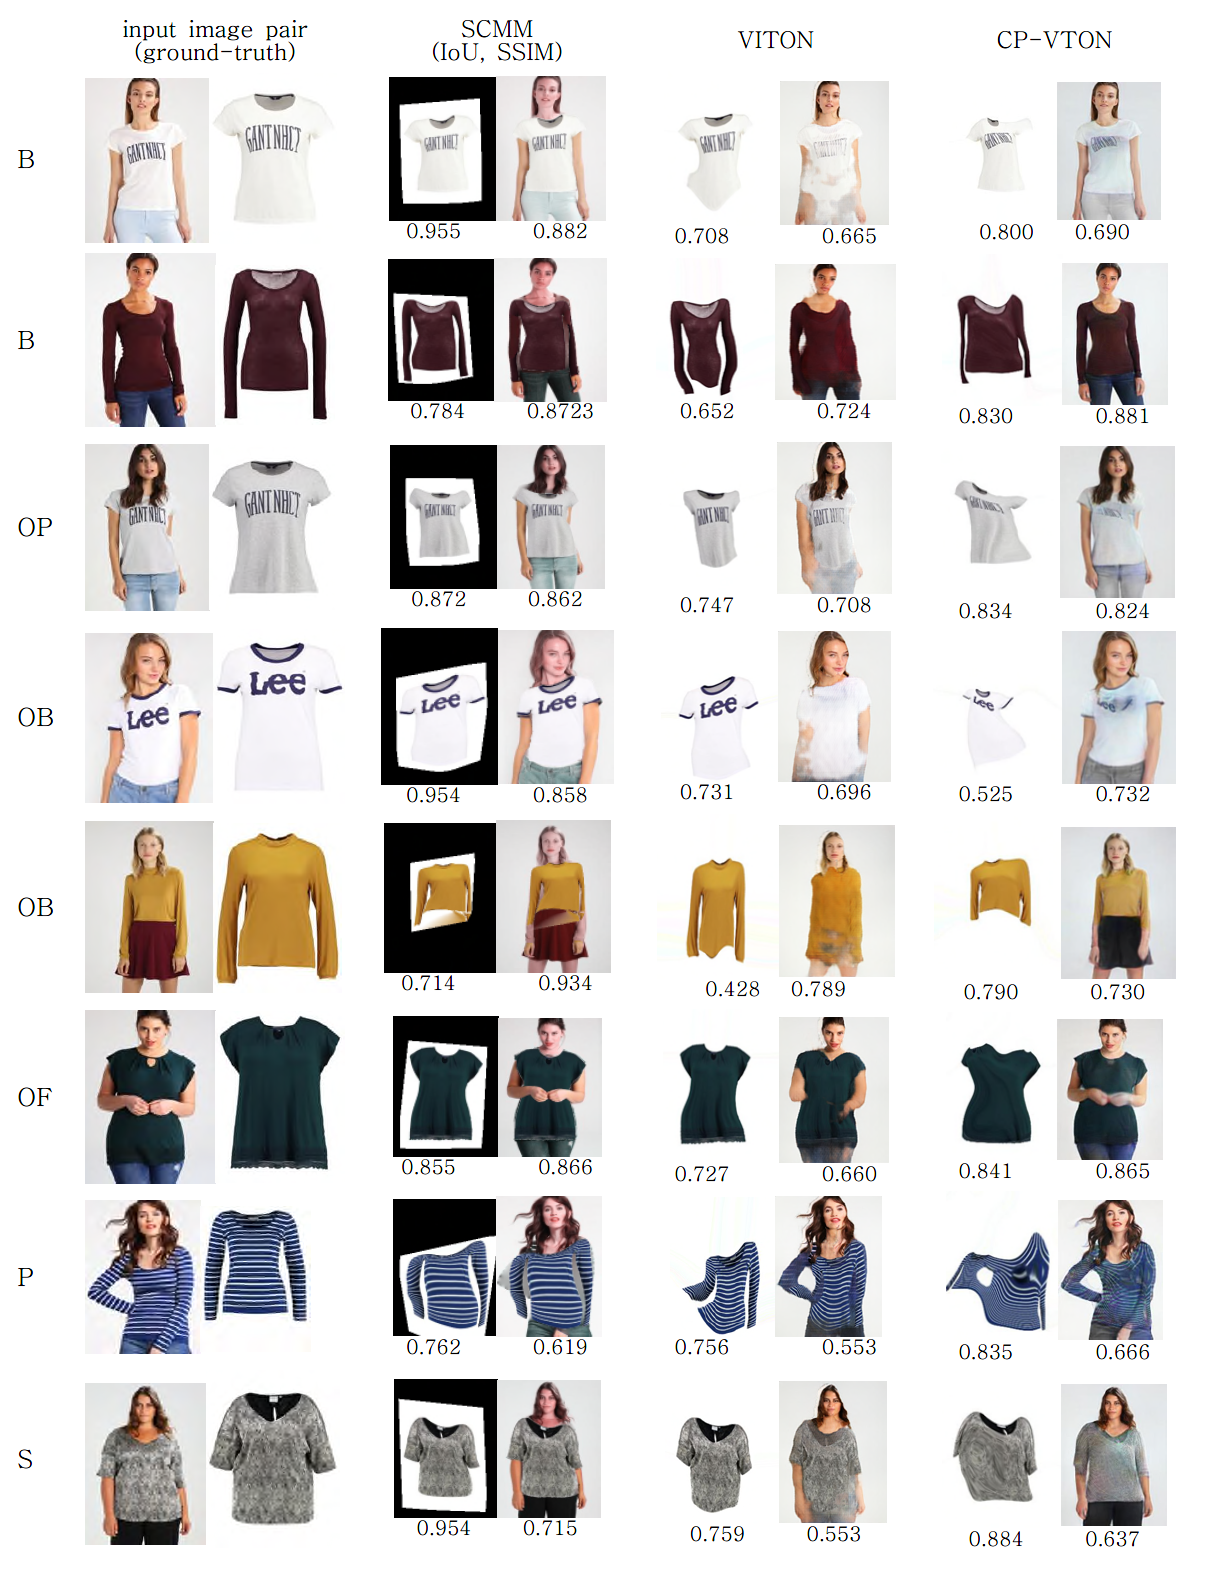
\includegraphics[height=13.5cm, scale=1]{figures/2dvton_same.png}   % TODO
\caption{Failures of 2D image-based cloth deformation for Virtual Try-On (Same clothes pairs)}
\label{fig:classified2DVTONresult}
\end{figure}



Especially note that the warped clothes are often too much different for trying on desired human body shapes. There are two main facts. Firstly, the 3D deformation that any 2D deformation including non-rigid transform such as TPS is quite limited, especially any 2D deformation cannot handle when the two area in the original image are overlapped in the destination images. Therefore, when the arms of long sleeved clothes occlude the main body, 2D warping methods cannot approximate the 3D deformation properly. Secondly, the deformation needs corresponding points between the source and target image. The clothes are extremely difficult objects to find the corresponding points. The Shape Context Matching (SCM\cite{BelongieMP02} and Spatial Transformer Networks (STN)\cite{JaderbergSZK15} based deformations cannot find the corresponding points when the target cloth and original cloth has different shapes. There are also other failure cases and issues of 2D image-based non-rigid deformations and virtual try-on applications, as we discussed in Section \ref{section:intro}. For example, CP-VTON\cite{Wang2018TowardCI} claims to preserve clothing characteristics, i.e., texture, color, shape etc. However, as shown in Figure \ref{fig:2dvtondiff}, that is not the case all the time. In conclusion, the 2D image-based algorithms has serious limitations in range of applications. It can be applied to the mild-posed target humans only and simple short-sleeved clothes, mainly because the inherent limitations of 2D deformation methods including non-rigid ones, and the poor performance of matching algorithm.  To overcome these limitations, we consider of modeling the try-on cloth into a 3D human body model, and apply the 3D deformations.


